\documentclass[a4paper]{report}


%%%%%%%% FONT %%%%%%%%
\usepackage[utf8]{inputenc}
\usepackage[T1,T2A,T5]{fontenc}
\usepackage{bookmark}
\usepackage{parskip}
%%%%%%%% MATH %%%%%%%%
\usepackage{amsmath}
\usepackage{amsthm}
\usepackage{a4wide,amssymb,epsfig,latexsym,array,hhline,fancyhdr}
\usepackage[normalem]{ulem}
\usepackage[export]{adjustbox}
\usepackage{amssymb}
\usepackage{mathtools}
\usepackage{float}
%%%%%%%% CODE %%%%%%%%
\usepackage{listings}
\usepackage{chngcntr}
%%%%%%%% COLOR %%%%%%%%
\usepackage{color}
\usepackage{xcolor, colortbl, rotating, multirow, booktabs, bigstrut}
\usepackage[makeroom]{cancel}
\usepackage{booktabs}
\usepackage{alltt}
\usepackage[framemethod=tikz]{mdframed}
\usepackage{caption,subcaption}
\usepackage{placeins}
\usepackage[lined,boxed,commentsnumbered]{algorithm2e}
\usepackage{enumerate}
%%%%%%%% GRAPHIC %%%%%%%%
\usepackage{graphicx}
\usepackage{graphics}
\usepackage{geometry}
\usepackage{tikz}
\usetikzlibrary{automata, positioning}
%%%%%%% TABLE %%%%%%%%
\usepackage{multicol,longtable,amscd}
\usepackage{tabularx, caption}
\usepackage{multirow}
\usepackage{multicol}
\usepackage[export]{adjustbox}
%%%%%%%% FORMAT %%%%%%%%
\usetikzlibrary{calc}
\usepackage{lastpage}
\usepackage{array}
\usepackage{rotating}
\usepackage{setspace}
\usepackage{epsfig}
\usepackage{blindtext}
\usepackage{enumitem}
%%%%%%%% HYPERREF %%%%%%%%
\usepackage{tabularray}
\usepackage{bm}
\usepackage{imakeidx}
\usepackage[flushleft]{threeparttable}
\usepackage{biblatex}
\usepackage[normalem]{ulem}
\usepackage{lipsum}

\usepackage{color,soul}
\definecolor{azure}{rgb}{0.0, 0.5, 1.0}
\newcommand{\markgray}[1]{\ignorespaces{\color{gray} #1}}
\newcommand{\markgreen}[1]{{\color{green!50!black} #1}}
\newcommand{\markred}[1]{{\color{red!80!black} #1}}
\newcommand{\markblue}[1]{{\color{azure!80!black} #1}}

\colorlet{llgray}{lightgray!40}

\newcommand\numberthis{\addtocounter{equation}{1}\tag{\theequation}}
\newcommand{\eg}{{\ignorespaces\emph{e.g.,}}{ }}
\newcommand{\ie}{{\ignorespaces\emph{i.e.,}}{ }}
\newcommand{\citesth}{\markgray{(cite something)}}

\newcommand{\refsth}{\markgray{(X)}}

\usepackage{aligned-overset}
\allowdisplaybreaks
\usepackage{cancel}

\usepackage{enumitem}
\usepackage{multirow}

\newcommand{\specialcell}[2][c]{%
  \begin{tabular}[#1]{@{}c@{}}#2\end{tabular}}

\usepackage{wrapfig}




\hypersetup{
  colorlinks,
  linkcolor={black},
  citecolor={blue!50!black},
  urlcolor={blue!50!black}
}
\usepackage{styles}
\usepackage{commands}


\hypersetup{colorlinks=true,urlcolor=blue,linkcolor=black,citecolor=black}
\makeindex[columns=3, title=Index, intoc]

\def\thesislayout{
	\geometry{
		a4paper,
		total={160mm,240mm}, 
		left=30mm,
		top=30mm,
	}
}
\thesislayout

\setlength{\headheight}{40pt}
\pagestyle{fancy}

\fancyhead[L]{}
\fancyhead[R]{\nouppercase{\textbf{\Roman{chapter}.\rightmark}}}

\renewcommand{\headrulewidth}{0.3pt}

\setcounter{secnumdepth}{4}
\setcounter{tocdepth}{3}
\makeatletter
\everymath{\color{blue}}

\sloppy
\captionsetup[figure]{labelfont={small,bf},textfont={small},belowskip=-1pt,aboveskip=-9pt}
\captionsetup[table]{labelfont={small,bf},textfont={small},belowskip=-1pt,aboveskip=7pt}

\setlength{\floatsep}{5pt plus 2pt minus 2pt}
\setlength{\textfloatsep}{5pt plus 2pt minus 2pt}
\setlength{\intextsep}{10pt plus 2pt minus 2pt}
\thesislayout

\everymath{\color{black}}

\thesislayout
% \addbibresource{refs.bib}

\author{}
\title{}
\date{}

\begin{document}
\counterwithin{lstlisting}{section}
\renewcommand{\thelstlisting}{\arabic{chapter}.\arabic{section}.\arabic{lstlisting}}

\begin{titlepage}
  \begin{tikzpicture}[remember picture, overlay]
    \draw[line width = 4pt] ($(current page.north west) + (2.5cm,-2cm)$) rectangle ($(current page.south east) + (-1.5cm,2cm)$);
  \end{tikzpicture}
  \begin{center}
    VIETNAM NATIONAL UNIVERSITY, HO CHI MINH CITY\\
    UNIVERSITY OF TECHNOLOGY\\
    FACULTY OF COMPUTER SCIENCE AND ENGINEERING
  \end{center}

  \vspace{1cm}

  \begin{figure}[ht]
    \centering
    
\includegraphics[width=5cm]{hcmut.png}
  \end{figure}

  \vspace{1cm}

  \begin{center}
    \begin{tabular}{c}
      \multicolumn{1}{c}{\textbf{{\Large \color{blue} PROBABILITY AND STATISTICS}}} \\ \\
      ~~                                                                            \\
      \hline
      \\
      \textcolor{black}{\textbf{{\Large THE EVOLUTION OF COMPUTER PROCESSORS:}}}    \\\\
      \textcolor{black}{\textbf{{\Large A STATISTICS OF COMMON PROPERTIES}}}        \\
      ~~                                                                            \\
      \hline
      \\
    \end{tabular}
  \end{center}

  \begin{table}[h]
    \begin{tabular}{rrll}

      \hspace{5 cm}
       & Instructor: & Dr. Nguyen Thi Mong Ngoc \\
       & Students:   & Chau Dang Minh - 2013748 \\
       &             &
    \end{tabular}
  \end{table}
  \vspace{2cm}
  \begin{center}
    {\footnotesize Ho Chi Minh City, May 2024}
  \end{center}
\end{titlepage}

\chapter*{Evaluation}
\begin{center}
 \begin{tabular}{|c|c|c|l|c|}
  \hline
  \textbf{N.O.} & \textbf{Student}   & \textbf{ID} & \textbf{Works}           & \textbf{Completed} \\
  \hline
  1             & Chau Dang Minh     & 2212287     & \begin{tabular}{@{}l@{}}
                                                      Dataset overview \\
                                                      Preprocessing
                                                     \end{tabular} & 100\%                       \\
  \hline
  2             & Ha Khoi Nguyen     & 2212287     & Descriptive statistics   & 100\%              \\
  \hline
  3             & Nguyen Thi Mai Anh & 2210103     & \begin{tabular}{@{}l@{}}
                                                      Theories \\
                                                      Slides and Presentation
                                                     \end{tabular} &                       \\
  \hline
  4             & Võ Ninh Giang      & 2210834     & \begin{tabular}{@{}l@{}}
                                                      Inferential statistics
                                                     \end{tabular} &                       \\
  \hline
  5             & Trinh Viet Cuong   & 2210447     & \begin{tabular}{@{}l@{}}
                                                      Inferential statistics
                                                     \end{tabular} &                       \\
  \hline
 \end{tabular}
\end{center}
\chapter*{Introduction and Acknowledgement}

Phenomena that are meaningful to humans appear not to be completely stochastic. In the same sense, datasets produced by humans, or nature in time circulations have insights to be analyzed, which is accounted by Statistics. Thanks to Dr. Nguyen Thi Mong Ngoc's supervision in Probability and Statistics course, we have a chance to study basic statistics within an assignment with a tiny dataset. We organized our report in the following structure

\begin{enumerate}
  \item Overview of the dataset. In this chapter, we carefully describe in details as much as possible the dataset, specifically the properties of each instance. We also notice which features to be used for later statistical tasks.
  \item Preprocessing. We process data cleaning and some computations.
  \item Descriptive statistics. We calculate some qualitative features of the dataset.
  \item Inferential statistics. Our problems are explicitly stated and solved.
\end{enumerate}
\tableofcontents
\chapter{Overview of the Dataset}

As Computer Science students, we are assigned to analyze a \href{https://www.kaggle.com/datasets/iliassekkaf/computerparts/data}{dataset about computer processors}, namely CPUs and GPUs. Our dataset is credited to Intel, Game-Debate, and the companies involved in producing the part. Information of CPUs and GPUs are collected separately into two files, namely \texttt{Intel\_CPUs.csv} and \texttt{All\_GPUs.csv}.


\chapter{Foundations}

A statistical Hypothesis is a statement or assumption about the parameters of one or more populations, which may be true or false. Each such truth value can be expressed in the form of a hypothesis, usually denoted as $H_0$, called the null hypothesis, and an alternative hypothesis, usually denoted as $H_1$ or Halt, which is its complement.

\section{Theory of Sampling}
\subsection{Terminology}
\begin{enumerate}
 \item A population is a set $\{x_i\}_{i=1}^N$ of elements belonging to the object under study, which need to be observed, collected, and analyzed based on certain characteristics. A parameter is a numerical description of a population.
 \item A sample is a subset $\{x_{i_j}\}_{j=1}^n$ of units selected from the population according to a certain sampling method. A statistic is a numerical description of a sample.
 \item Let the population belong to a distribution represented by a random variable $X$. A random sample is a collection $\{X_i\}_{i=1}^n$ such that $X,X_1,\ldots,X_n$ are independent and identically distributed.
\end{enumerate}

\subsection{Statistical characteristics}

Statistical characteristics are important properties on a population, a sample or a random sample directly related to the content of the study and survey, which need to be collected from the units of the population, generally divided into two groups

\begin{enumerate}
 \item Central tendency includes mean, median, mode, giving us an idea of the trend of the data points clustering around certain values.
 \item Dispersion includes variance, standard deviation, which describe the spread or variability of the data points around the central tendency.
\end{enumerate}

In details, these quantities are formulated as followings.
\begin{enumerate}
 \item Population mean
       \begin{equation}
        \mu = \frac{1}{N} \sum_{i=1}^N x_i.
       \end{equation}
 \item Sample mean
       \begin{equation}
        \bar{x} = \frac{1}{n} \sum_{j=1}^n x_{i_j}.
       \end{equation}
 \item Random sample mean
       \begin{equation}
        \bar{X} = \frac{1}{n} \sum_{i=1}^n X_i.
       \end{equation}
 \item Population variance
       \begin{equation}
        \sigma^2 = \dfrac{1}{N} \sum_{n=1}^N (x_n - \bar{x})^2.
       \end{equation}
 \item Sample variance
       \begin{equation}
        s^2 = \dfrac{1}{n-1} \sum_{j=1}^n (x_{i_j} - \bar{x})^2.
       \end{equation}
 \item Random sample variance
       \begin{equation}
        S^2 = \dfrac{1}{N-1} \sum_{n=1}^n (X_i - \bar{X})^2.
       \end{equation}
 \item Population, sample and random sample derivations are the square roots $\sigma$, $s$ and $S$, respectively.

 \item Sample ratio
       \begin{equation}
        f = \dfrac{n}{N}
       \end{equation}
 \item Coefficient of variation
       \begin{equation}
        \mathrm{CV} = \left(\frac{s}{\bar{x}}\right) \cdot 100\%
       \end{equation}
 \item Suppose that the sample $\{x_{i_j}\}_{j=1}^n$ is in increasing order. The sample median is calculated as
       \begin{equation}
        \mathrm{med} = \begin{cases}
         x_{i_{k+1}},                            & \text{ if } n = 2k+1 \\
         \dfrac{1}{2} (x_{i_{k}} + x_{i_{k+1}}), & \text{ if } n = 2k.
        \end{cases}
       \end{equation}
 \item Quartiles include three values $Q_1,Q_2$ and $Q_3$. Where $Q_2$ is the median, $Q_1$ and $Q_3$ is the median of the set of samples less than and more than $Q_2$, respectively. The quantity $\mathrm{IQR} = Q_3-Q_1$ is called the interquartile range.
 \item An outlier is a point outsize $(Q1 - 1.5 \times IQR, Q3 + 1.5 \times IQR)$.
\end{enumerate}

\section{Statistical Hypothesis Testing}
The process of testing a statistical hypothesis is a standardized procedure for making decisions to reject or not reject a hypothesis based on sample data. This process is called hypothesis testing and typically involves four steps:

\begin{enumerate}
 \item \textbf{Setting Hypotheses} involves stating which hypothesis is null and which is alternative. The hypotheses are formulated in a mutually exclusive manner, meaning if one is true, the other must be false.
 \item \textbf{Constructing an Analysis Plan} outlines how sample data will be used to evaluate the null hypothesis. Evaluation typically centers around a single test statistic.
 \item \textbf{Analyzing Sample Data} determines the values of the sample statistic (mean, proportion, $t$-statistic, $z$-score, etc.) as described in the analysis plan.
 \item \textbf{Interpreting Results} applies decision rules outlined in the analysis plan. If the observed result is inconsistent with the null hypothesis, reject it.
\end{enumerate}

Similar to estimation, statistical hypothesis testing does not provide results with 100\% certainty but rather with a certain level of confidence, and errors can occur. Errors can be classified into two types:

\begin{itemize}
 \item \textbf{Type I Error:} Rejecting the null hypothesis $H_0$
       and accepting the alternative hypothesis $H_1$ whereas $H_0$ is true.
 \item \textbf{Type II Error:} Failing to reject the null hypothesis $H_0$ and not accepting the alternative hypothesis $H_1$ whereas $H_1$ is true.
\end{itemize}

Both types of errors can have adverse consequences. Depending on the situation, it's assessed which type of error leads to more serious consequences and should be minimized.

To make decisions about rejecting the null hypothesis, statisticians rely on specific rules. These rules are listed in the analysis plan. Traditionally, statisticians describe these decision rules in two ways: referencing a p-value or referencing a region of acceptance.

\begin{itemize}
 \item \textbf{$p$-value:} The strength of evidence in favor of a null hypothesis is measured by the $p$-value. Suppose the test statistic is denoted by S. The $p$-value is the probability of observing a test statistic as extreme as $S$, assuming the null hypothesis is true. If the $p$-value is smaller than the significance level, we reject the null hypothesis.
 \item \textbf{Region of Acceptance:} The region of acceptance is a range of values. If the sample statistic falls within the region of acceptance, the null hypothesis is not rejected. The region of acceptance is set so that the probability of committing a Type I error is equivalent to the significance level.
\end{itemize}

Values outside the region of acceptance are called the region of rejection. If the sample statistic falls within the region of rejection, the null hypothesis is rejected. In such cases, it's said that the null hypothesis has been rejected at the  significance level.

\section{Linear Regression}
Linear regression constructs a linear model between independent variables $\mathbf{x}=(0, x_1,\ldots, x_d)\in\RR^{d+1}$ and a dependent variable $y\in\RR$. Traditionally, the relation is expressed as

\begin{equation}
 \begin{aligned}
  y
   & = w_0 + \sum\limits_{i=1}^n w_ix_i \\
   & = \mathbf{x}^\top\mathbf{w},
 \end{aligned}
\end{equation}

where $\{w_i\}_{i=0}^d$ are parameters to learn. Let $\{(\mathbf{x}_n, \hat{y}_n)\}_{n=1}^N$ be collected observations. Our objective is to minimize the error
\begin{equation}
 \begin{aligned}
  \L(\mathbf{w})
   & = \sum\limits_{n=1}^N (y-\hat{y})^2                                                              \\
   & = \sum\limits_{n=1}^N (\mathbf{w}^\top \mathbf{x}_n-\hat{y}_n)^2                                 \\
   & = \|\mathbf{X} \mathbf{w} - \hat{\mathbf{y}}\|^2                                               ,
 \end{aligned}
\end{equation}
where $\hat{\mathbf{y}} = (\hat{y}_1,\ldots,\hat{y}_n)^\top \in \RR^n$ and $\mathbf{X} = (\mathbf{x}_1,\ldots,\mathbf{x}_n)\in\RR^{n\times(d+1)}$.
Taking the derivative of $\L$, we have
$$\dfrac{\d\L(\mathbf{w})}{\d \mathbf{w}} = 2\mathbf{X}^\top(\mathbf{X} \mathbf{w} - \hat{\mathbf{y}}).$$

Equivalently, $\mathbf{X}^\top \mathbf{X} \mathbf{w} =  \mathbf{X}^\top\hat{\mathbf{y}}$. If $\mathbf{X}^\top \mathbf{X}$ is invertible i.e. the independent variables are linearly independent, we have the unique solution
\begin{equation}
 \mathbf{w} = (\mathbf{X}^\top \mathbf{X})^{-1}\mathbf{X}^\top\hat{\mathbf{y}}.
\end{equation}

Along with the independence of independent variables, some requirements need to be satisfies for an accurate and reliable solution.

\begin{enumerate}
 \item  Linearity: The independent and dependent variables correlate. This means that the change in one or more independent variables induces the change in the dependent variable.
 \item Independence: The observed data in the dataset are independent of each other. This means that the value of the dependent variable for one observed data point does not depend on the value of the dependent variable for another observed data point.
 \item Across all levels of the independent variables, the variance of the errors remains constant. This indicates that the number of independent variables does not affect the variability of the errors.
 \item Normality: The errors in the model follow a normal distribution.
\end{enumerate}

% \subsubsection{Hai loại hồi quy tuyến tính}

% \textbf{- Hồi quy tuyến tính đơn: }\\
% + Nếu một biến độc lập duy nhất được sử dụng để dự đoán giá trị của một biến phụ thuộc số, thì thuật toán hồi quy tuyến tính như vậy được gọi là Hồi quy tuyến tính đơn.\\
% + Giá trị kỳ vọng của $Y$ ở mỗi mức $x$ là biến ngẫu nhiên $E(Y|x) = \beta_0 + \beta_{1}x$. Ta cho rằng mỗi biến $Y$ có thể được mô tả bằng mô hình $Y = \beta_0 + \beta_{1}x + \varepsilon$.\\
% + Trong đó: $Y$ là biến độc lập, $\beta_0$ là giao điểm của $Y$ khi $x$ bằng 0, $\beta_1$ là hệ số của $x$, $\varepsilon$ là hệ số độc lập của mô hình.\\
% + Tức là $Y_i = \beta_0 + \beta_{1}x_i + \varepsilon_i $ với $i=1,2,...,n$.\\
% + Để đạt được đường hồi quy phù hợp nhất, điều cần thiết là phải đưa ra dự đoán giá trị mà sự khác biệt giữa giá trị dự đoán và giá trị thực $Y$ là nhỏ nhất. Vì vậy, chúng ta phải thay đổi giá trị của $\beta_0,  \beta_{1}$ , để đạt được giá trị tốt nhất của cả hai.

% \textbf{- Hồi quy tuyến tính bội:}\\
% + Nếu sử dụng nhiều hơn một biến độc lập để dự đoán giá trị của một biến phụ thuộc số lượng thì thuật toán hồi quy tuyến tính như vậy được gọi là Đa tuyến tính hồi quy.\\
% + Giá trị kỳ vọng của $Y$ ở mỗi mức $x$ là biến ngẫu nhiên $E(Y|x) = \beta_0 + \beta_{1}x_1 + ... + \beta_{i}x_i$. Ta cho rằng mỗi biến $Y$,
% có thể được mô tả bằng mô hình $Y = \beta_0 + \beta_{1}x_1 + ... + \beta_{i}x_i \varepsilon_i $.\\
% + Trong đó: $Y$ là biến độc lập, $\beta_0$ là giao điểm của $Y$ khi $x$ bằng 0, $\beta_1$ là hệ số của $x$, $\varepsilon$ là hệ số độc lập của mô hình.\\
% + Tức là $Y_i = \beta_0 + \beta_{1}x_1 + ... + \beta_{i}x_i  \varepsilon_i $ với $i=1,2,...,n$.\\

% \subsubsection{Định nghĩa hồi quy từng bước}

% - Hồi quy từng bước là một phương pháp điều chỉnh mô hình hồi quy bằng cách lặp đi lặp lại, thêm hoặc loại bỏ các biến. Nó được sử dụng để xây dựng một mô hình chính xác và chi tiết, có nghĩa là nó có số lượng biến nhỏ nhất có thể giải thích dữ liệu.

% - Có hai loại hồi quy từng bước là:\\
% + Lựa chọn chuyển tiếp: Thuật toán bắt đầu với một mô hình trống và lặp đi lặp lại hoặc thêm các biến vào mô hình cho đến khi không có cải tiến nào nữa.\\
% + Loại bỏ ngược: Thuật toán bắt đầu với một mô hình bao gồm tất cả các biến và loại bỏ lặp đi lặp lại các biến cho đến khi không còn cải tiến nào nữa.\\
% + Ưu điểm của hồi quy từng bước là nó có thể tự động chọn các biến quan trọng nhất cho mô hình và xây dựng một mô hình chi tiết. Điểm bất lợi là nó không phải lúc nào cũng chọn được mô hình tốt nhất và có thể nhạy cảm với thứ tự các biến được thêm vào hoặc loại bỏ.
% \subsubsection{Hồi quy từng bước và hồi quy tuyến tính}

% - Hồi quy tuyến tính là một phương pháp thống kê được sử dụng để mô hình hóa mối quan hệ giữa một biến phụ thuộc và một hoặc nhiều biến độc lập bằng cách khớp phương trình tuyến tính với dữ liệu quan sát được. Nói cách khác, đây là phương pháp dự đoán phản hồi (hoặc biến phụ thuộc) dựa trên một hoặc nhiều biến dự đoán.

% - Hồi quy từng bước là phương pháp xây dựng mô hình hồi quy bằng cách thêm hoặc loại bỏ các yếu tố dự đoán theo kiểu từng bước. Mục tiêu của hồi quy từng bước là xác định tập hợp con các yếu tố dự đoán mang lại hiệu suất dự đoán tốt nhất cho biến phản hồi. Điều này được thực hiện bằng cách bắt đầu với một mô hình trống và lặp đi lặp lại việc thêm hoặc loại bỏ các yếu tố dự đoán dựa trên mức độ mối quan hệ của chúng với biến phản hồi.

% - Tóm lại, hồi quy tuyến tính là phương pháp mô hình hóa mối quan hệ giữa phản hồi và một hoặc nhiều biến dự đoán, trong khi hồi quy từng bước là phương pháp xây dựng mô hình hồi quy bằng cách lặp đi lặp lại thêm hoặc loại bỏ các yếu tố dự đoán.

\section{Analysis of Variance}

Analysis of Variance (ANOVA) is a statistical analysis tool used to partition the total observed variability found in a dataset into two parts: Systematic factors and Random factors. Systematic factors statistically influence a certain dataset, while random factors do not. We use ANOVA to determine the influence of independent variables on the dependent variable in regression studies.

The T-Test and Z-Test methods, developed in the 20th century, were used for statistical analysis until 1918 when Ronald Fisher introduced the Analysis of Variance method. Both serve as hypothesis tests to assess whether there is any significant difference between means. The T-Test is used when the population variance is unknown or the sample size is small $(n < 30)$. Meanwhile, the Z-Test is applied when the population variance is known and the sample size is large $(n > 30)$. The T-Test uses the Student's t-distribution, while the Z-Test uses the standard normal distribution. As the sample size increases, the T-distribution converges to the standard normal distribution. The T-Test can be understood as a statistical test used to compare and analyze whether the mean values of two populations are different when the standard deviation is unknown. Conversely, the Z-Test is a parametric test applied when the standard deviation is known to determine whether the means of two datasets are different. ANOVA is also known as Fisher's analysis of variance and is an extension of both T-Tests and Z-Tests.

\subsection{ANOVA Usecases}

ANOVA test is the initial step in analyzing factors influencing a specific dataset. Upon completing a test, additional checks on measurable methodological factors contributing to dataset inconsistency are conducted. The results, using $F$-distribution, can be utilized to generate supplementary data suitable for proposed regression models.

ANOVA test enables comparison of more than two groups simultaneously to determine whether a relationship exists among them. The outcome of ANOVA analysis, the F-statistic (also known as the F-ratio), allows for analysis across multiple datasets to ascertain variation between samples and within samples.

If no significant differences exist among the tested groups (known as the null hypothesis), the $F$-statistic result of ANOVA will be close to $1$. The distribution of all possible values of the F-statistic follows the $F$-distribution. This is a family of probability distributions characterized by two parameters, known as the degrees of freedom of the numerator and the degrees of freedom of the denominator.

\subsection{Types of ANOVA}

There are two main types of ANOVA: one-way ANOVA and two-way ANOVA. Additionally, there are variations of ANOVA such as  Multivariate ANOVA (MANOVA), which differs from ANOVA in that the former tests multiple dependent variables simultaneously while the latter evaluates only one dependent variable at a time. One-way or two-way refers to the number of independent variables in the analysis of variance. Furthermore, ANOVA relies on assumptions. ANOVA tests assume that the data are normally distributed, the variance is nearly equal across groups, and all observations are independent. If these assumptions are not met, ANOVA may not be useful for group comparisons.

\subsubsection{One-way ANOVA}
One-way ANOVA is used to assess the effect of a single factor on a single response variable. It determines whether all samples are similar i.e. determine whether there is a statistically significant difference between the means of three or more independent (unrelated) groups. One-way ANOVA is formulated as
\begin{equation}
 Y_{i,j}=\mu_j + \varepsilon_{i,j},
\end{equation}
where $i=1,\ldots,n_j$ are indices of observations within the same group, $j=1,\ldots,k$ are indices of influenced groups, $\mu_j$ s the mean for each affected group and $\varepsilon_{i,j} \sim N(0,\sigma^2)$ is normal-distributed errors, independent for all $i$ and $j$. Mean and variance of $Y_{i,j}$ are $E(Y_{i,j})=\mu_j$ and $Var(Y_{i,j})=\sigma^2$, respectively.

\subsubsection{Two-way ANOVA}

Two-way ANOVA is an extension of one-way ANOVA, where there are two independent factors. It is used to observe the interaction between two factors and test the effects of two factors simultaneously. It is formulated as
\begin{equation}
 Y_{i,j}=\mu_j+\gamma_j+(\mu\gamma){i,j}+\varepsilon{i,j,k}.
\end{equation}
Assumptions about random variables are similar to one-way ANOVA.

\chapter{Preprocessing}

\section{Data Cleaning}

With \texttt{RStudio}, the working directory is automatically determined. Otherwise, it can be indicated by \texttt{here} library.

\begin{lstlisting}[caption={Required libraries and working directory setup}]
  # Libraries and options
  library(dplyr)
  library(here)
  library(knitr)
  library(kableExtra)
  
  # Self-defined functions
  source("utils.R")
  
  # Working directory
  setwd(here())
  \end{lstlisting}

Now our working directory have been explicated, we can use relative paths to read the data. With \texttt{RMarkdown}, we can prettify the rendering.

\begin{lstlisting}[caption={RStudio data object initialization}]
    # Read the CSV file into a data frame
    cpu_data <- read.csv("dataset/Intel_CPUs.csv")
    gpu_data <- read.csv("dataset/All_GPUs.csv")
    
    # Inspect the CPU data
    kable(head(cpu_data), format = "html") %>%
      kable_styling()
    \end{lstlisting}

\begin{figure}[!ht]
  \centering
  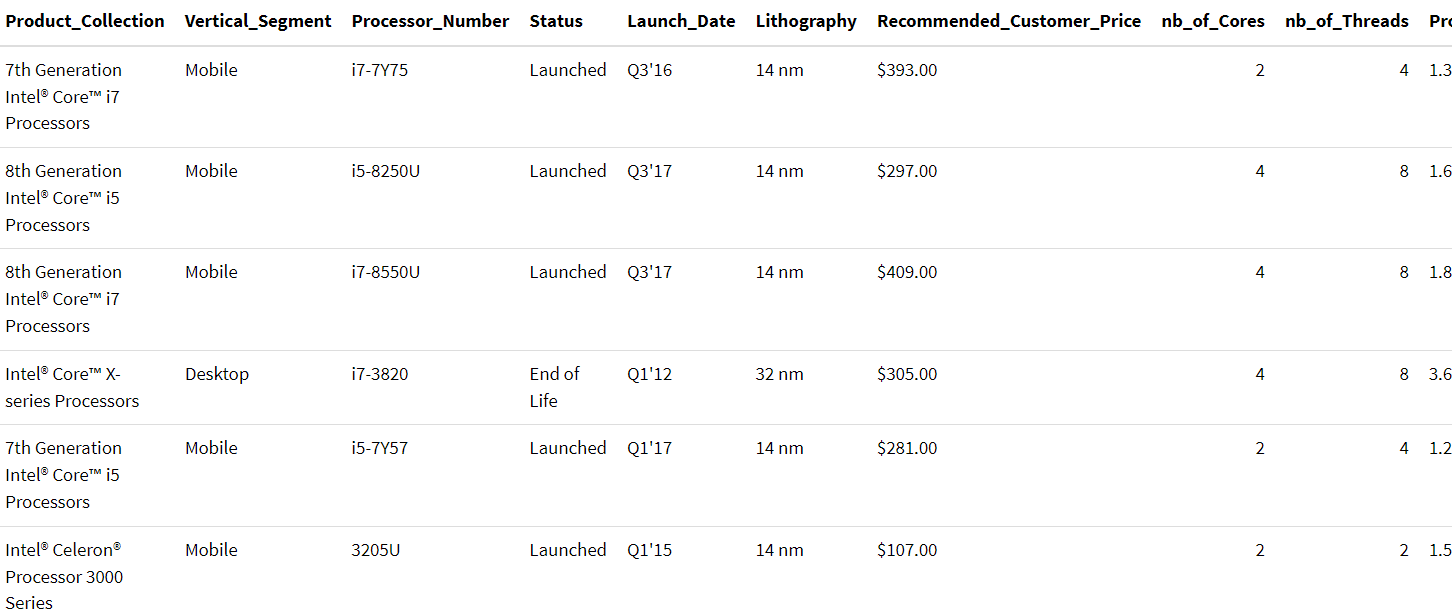
\includegraphics[width=\textwidth]{img/cpu-head.png}
  \vspace{0.5cm}
  \caption{First instances of CPUs data}
\end{figure}

Invalid cells may contain \texttt{NA}, an empty string, or other values showing us that this cell's data was not collecting correctly. At the very first step, we want to selected only columns whose the percentage of valid cells exceeds our predefined value. Then we filter out all instances with invalid features. Note that careful column selection possibly remains more instances for later tasks.

\begin{lstlisting}[caption={Cleaning functions}]
  # Check if a cell has a valid value
  is_valid <- function(value) {
    return(!is.na(value)
           & !is.null(value)
           & !value == ""
           & !value == "N/A"
           & !value == "-"
           & !value == "missing"
           & !value == "unknown")
    # Add your criteria
  }
  
  # Select columns with enough valid cells
  filtered_data <- function(data, valid_percentage=0.8) {
  selected_columns <- character(0) 
  
  for (col in colnames(data)) { 
    valid_count <- sum(is_valid(data[[col]])) 
    total_instances <- length(data[[col]]) 
    
    if ((valid_count / total_instances) >= fill) {
      selected_columns <- c(selected_columns, col)
    }
  }
  
  return(data[selected_columns])
}
  \end{lstlisting}


\begin{lstlisting}[caption={Cleaned data and selected features}]
  filtered_cpu_data <- filtered_data(cpu_data, 0.4)

  processed_cpu_data <- 
    filtered_cpu_data[
      apply(filtered_cpu_data, 1, function(row) all(sapply(row, is_valid))), ]
  
  selected_cpu_data <- processed_cpu_data[, c("Recommended_Customer_Price",
                                              "Product_Collection",
                                              "Launch_Date",
                                              "nb_of_Cores",
                                              "nb_of_Threads", 
                                              "Processor_Base_Frequency",
                                              "Bus_Speed")]
  
  # Adjust selected columns for your later needs

  kable(head(selected_cpu_data), format = "html") %>%
  kable_styling()
\end{lstlisting}

\begin{figure}[!ht]
  \centering
  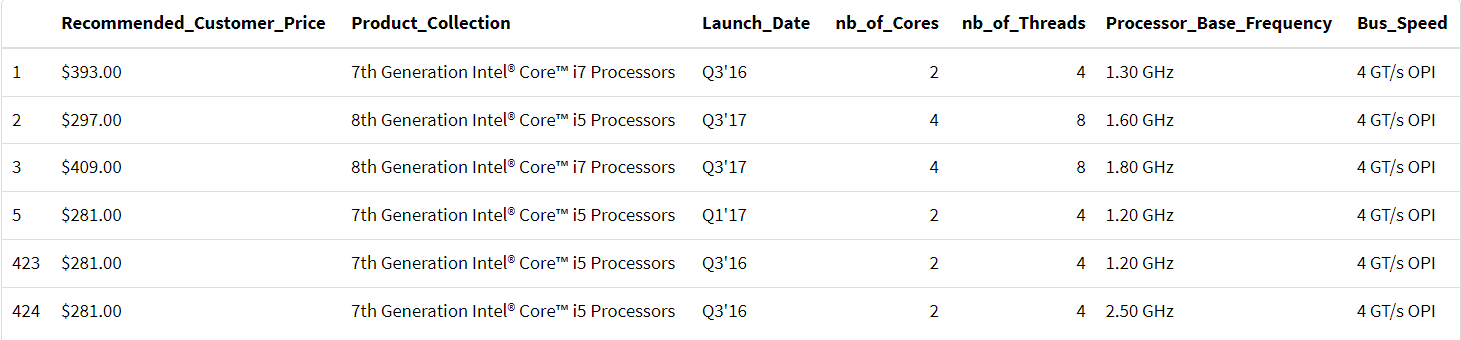
\includegraphics[width=\textwidth]{img/cpu-selected-head.png}
  \vspace{0.5cm}
  \caption{First instances of selected CPUs data}
\end{figure}

\section{Data Pre-computation}

Some features in our data have values that need to be reformatted for easily later sorting and analyses. Therefore, we need to gain a good understand on the features.


\begin{lstlisting}[caption={A processing for selected features}]
  cpu_columns <- colnames(cpu_data)
  gpu_columns <- colnames(gpu_data)
  intersect(cpu_columns, gpu_columns)
  # Output: character(0)
\end{lstlisting}

Since the data files have no common features, let us take a look at them independently.
\chapter{Descriptive Statistics}

\section{CPU Data}
\begin{figure}[p]
  \centering
  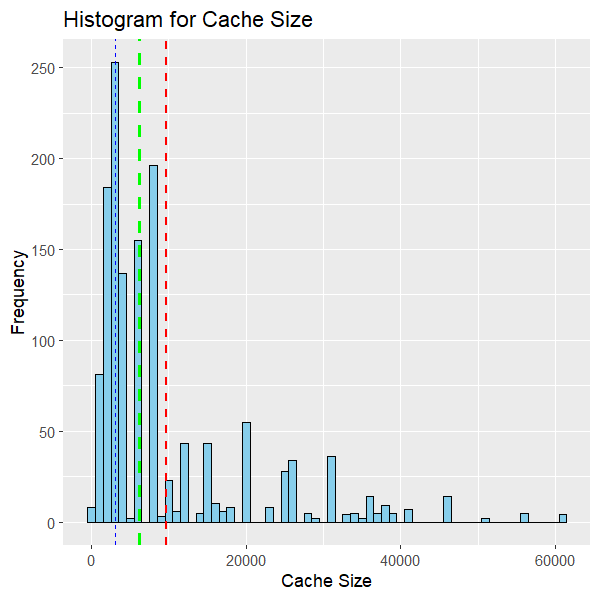
\includegraphics[width=0.33\linewidth]{img/CPU_histo_Cache.png}\hfill
  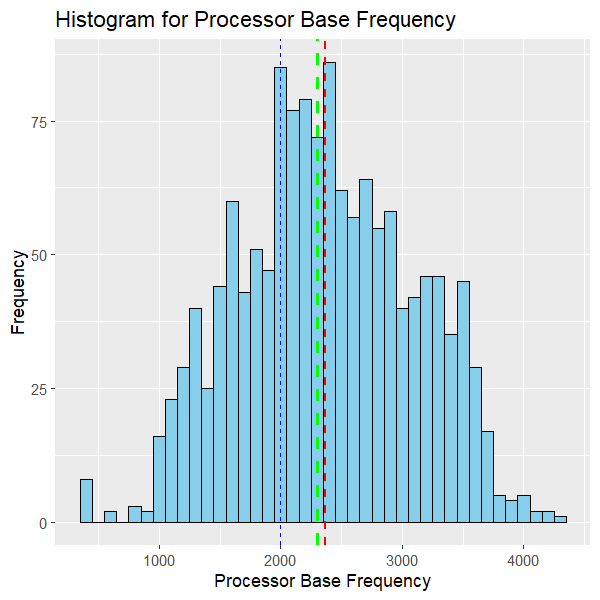
\includegraphics[width=0.33\linewidth]{img/CPU_histo_Freq.png}\hfill
  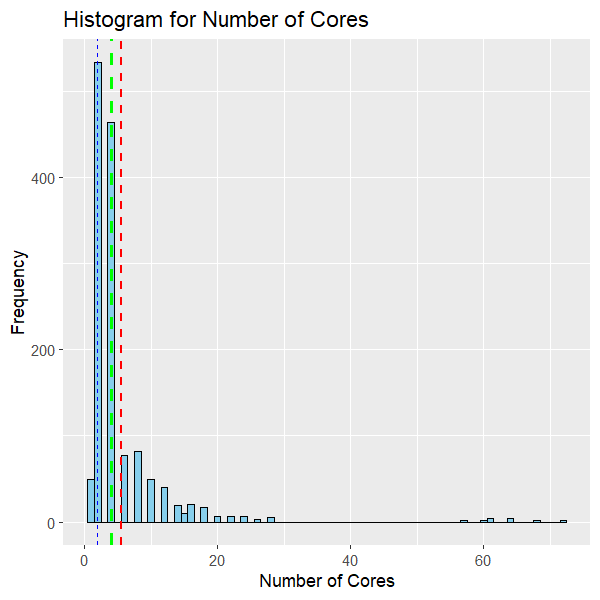
\includegraphics[width=0.33\linewidth]{img/CPU_histo_Core.png}
  \\[\smallskipamount]
  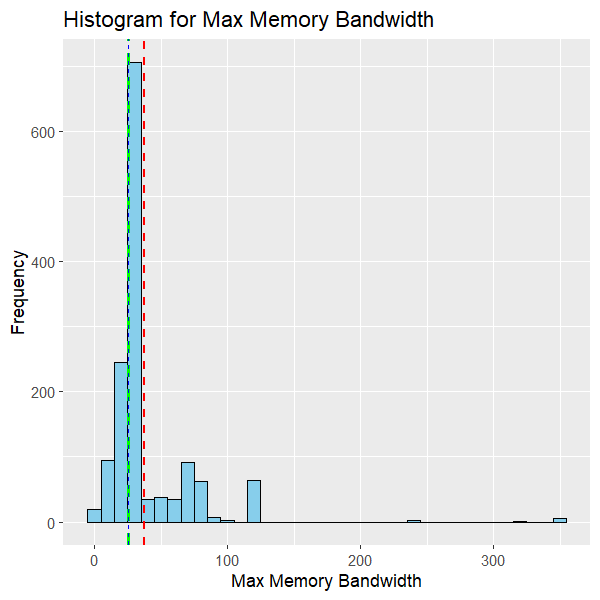
\includegraphics[width=0.33\linewidth]{img/CPU_histo_MMB.png}\hfill
  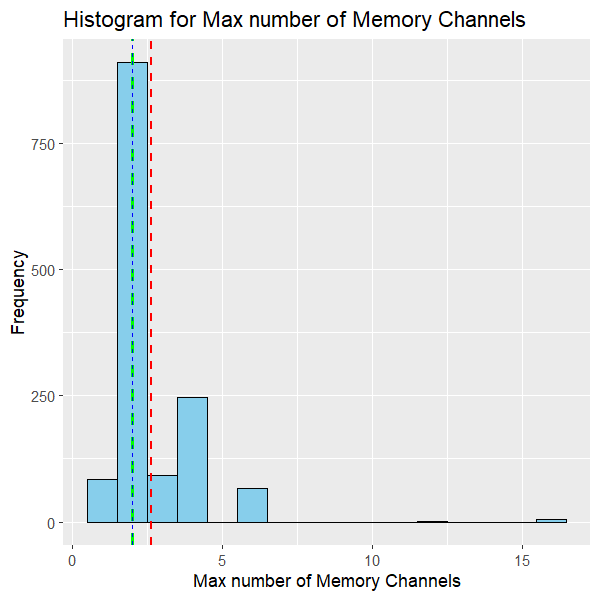
\includegraphics[width=0.33\linewidth]{img/CPU_histo_MNMC.png}\hfill
  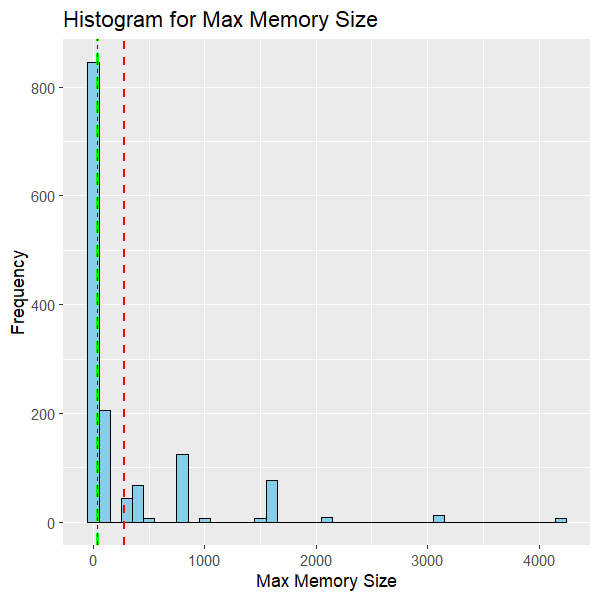
\includegraphics[width=0.33\linewidth]{img/CPU_histo_MMS.png}
  \\[\smallskipamount]
  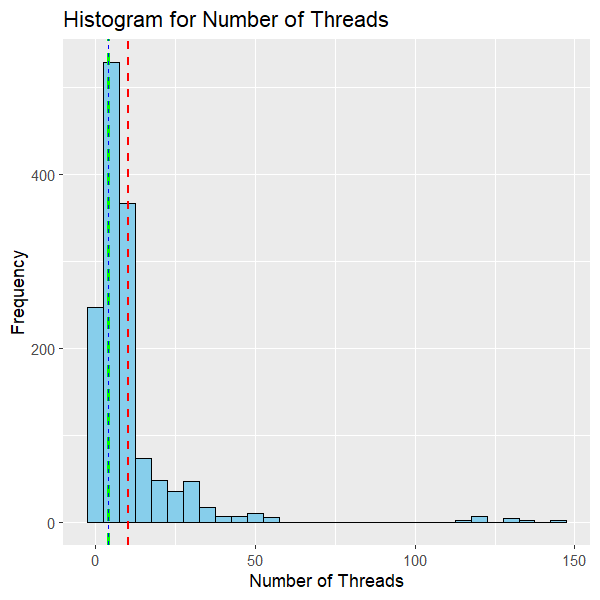
\includegraphics[width=0.33\linewidth]{img/CPU_histo_Thread.png}\hfill
  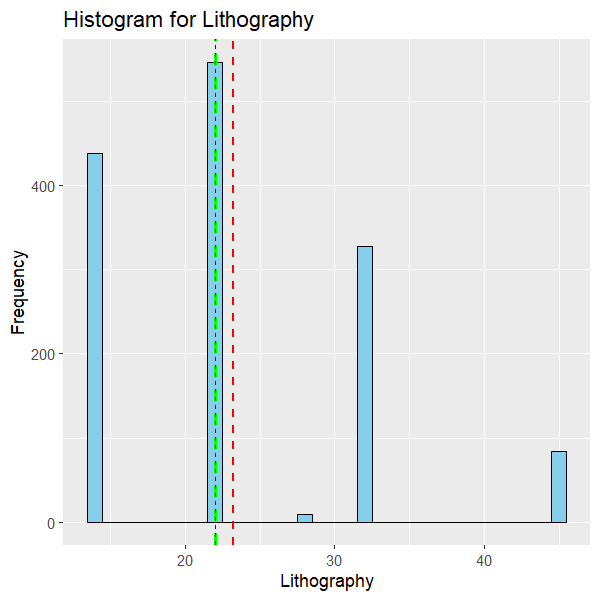
\includegraphics[width=0.33\linewidth]{img/CPU_histo_Litho.png}\hfill
  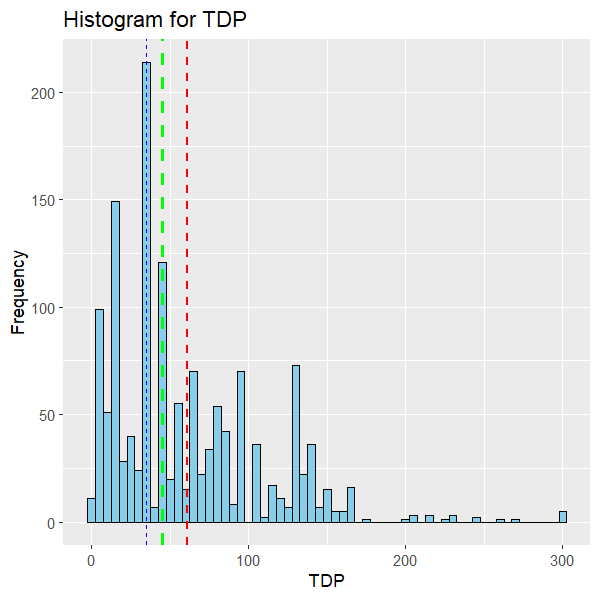
\includegraphics[width=0.33\linewidth]{img/CPU_histo_TDP.png}
  \vspace{10pt}
  \caption{Histograms of several features in CPU data}
  \label{fig:Na_GPU}
\end{figure}


\begin{lstlisting}[language=R]
litho_year <- CPUs_processed %>% 
  group_by(Release_Year) %>%
  summarize(mean_litho = mean(Lithography),
            median_litho = median(Lithography),
    .groups = "drop"
  )

ggplot(litho_year, aes(x = Release_Year)) +
  geom_line(aes(y = mean_litho, color = "Mean")) +
  geom_line(aes(y = median_litho, color = "Median")) +
  scale_color_manual(values = c("Mean" = "blue", "Median" = "red")) +
  labs(x = "Year", y = "Lithography", title = "Mean and Median Lithography by Year") +
  scale_x_continuous(breaks = seq(min(litho_year$Release_Year), max(litho_year$Release_Year),
  by = 1)) +
  theme_minimal()
\end{lstlisting}

\begin{figure}[ht]
  \centering
  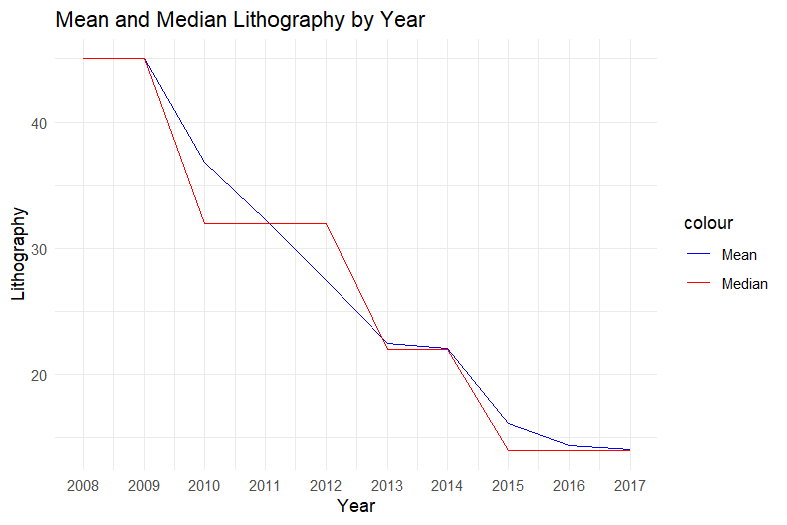
\includegraphics[width=1\linewidth]{img/Litho_Year.png}
  \vspace{1pt}
  \caption{Mean and median of lithography over years}
\end{figure}

\begin{lstlisting}[language=R]
options(repr.plot.width = 15, repr.plot.height =8) 
ggplot(data = CPUs_processed, aes(y = Status, x = Launch_Year, fill = Status)) +
  geom_boxplot() +
  labs(x = "Status", y = "Launch Date",title = "Boxplot of Status over Year") +
  scale_x_continuous(breaks = seq(min(Litho_year$Launch_Year), max(Litho_year$Launch_Year), by = 1))
\end{lstlisting}


\begin{figure}[ht]
  \centering
  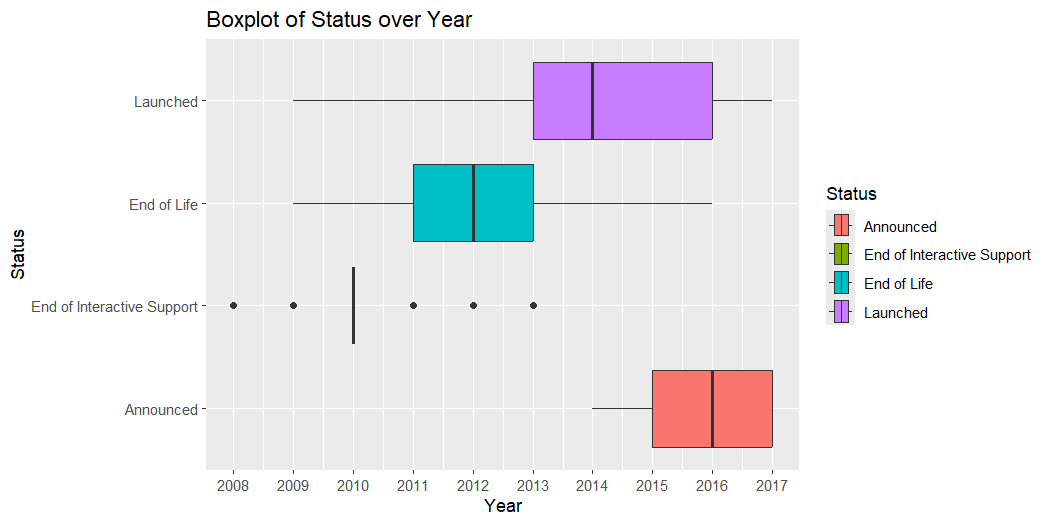
\includegraphics[width=1\linewidth]{img/Status_Year.png}
  \vspace{1pt}
  \caption{Status over years}
\end{figure}

\begin{lstlisting}[language=R]
options(repr.plot.width = 15, repr.plot.height =8) 
ggplot(data = CPUs_processed, aes(y = Vertical_Segment, x = Launch_Year, fill = Vertical_Segment)) +
  geom_boxplot() +
  labs(x = "Year", y = "Vertical Segment",title = "Boxplot of Vertical Segment over Year") +
  scale_x_continuous(breaks = seq(min(Litho_year$Launch_Year), max(Litho_year$Launch_Year), by = 1))
\end{lstlisting}

\begin{figure}[ht]
  \centering
  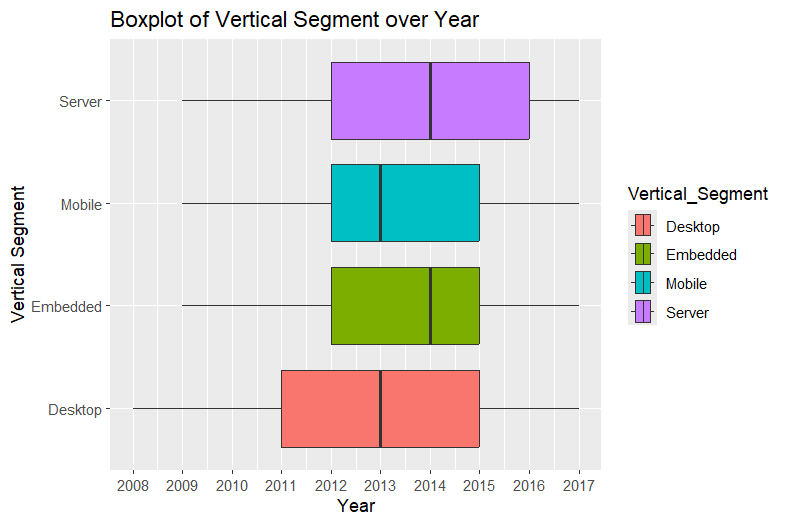
\includegraphics[width=1\linewidth]{img/VSegment_Year.png}
  \vspace{1pt}
  \caption{Segment over years}
\end{figure}

\begin{lstlisting}[language=R]
options(repr.plot.width = 15, repr.plot.height =8) 
ggplot(data = CPUs_processed, aes(y = Instruction_Set, x = Launch_Year, fill = Instruction_Set)) +
  geom_violin() +
  labs(x = "Launch Date", y = "Instruction set",title = "Violinplot of Instruction set over Year") +
  scale_x_continuous(breaks = seq(min(Litho_year$Launch_Year), max(Litho_year$Launch_Year), by = 1))
\end{lstlisting}

\begin{figure}[ht]
  \centering
  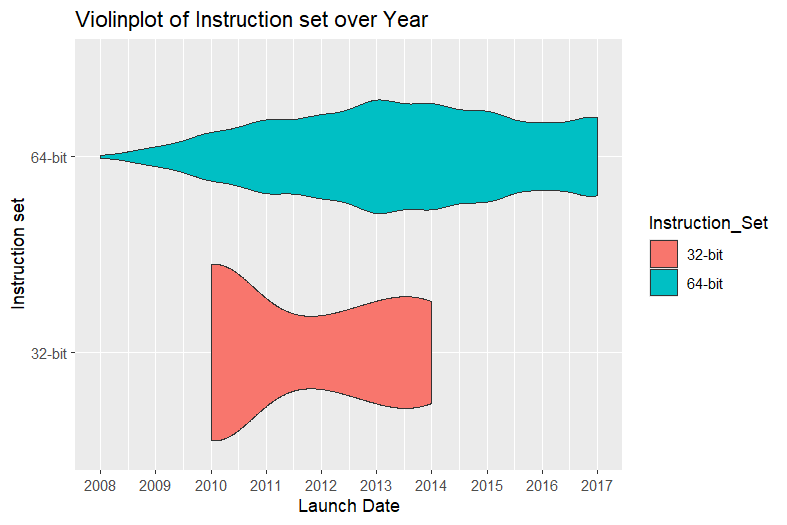
\includegraphics[width=1\linewidth]{img/6432bit_year.png}
  \vspace{1pt}
  \caption{Instruction set over years}
\end{figure}

\begin{figure}[ht]
  \centering
  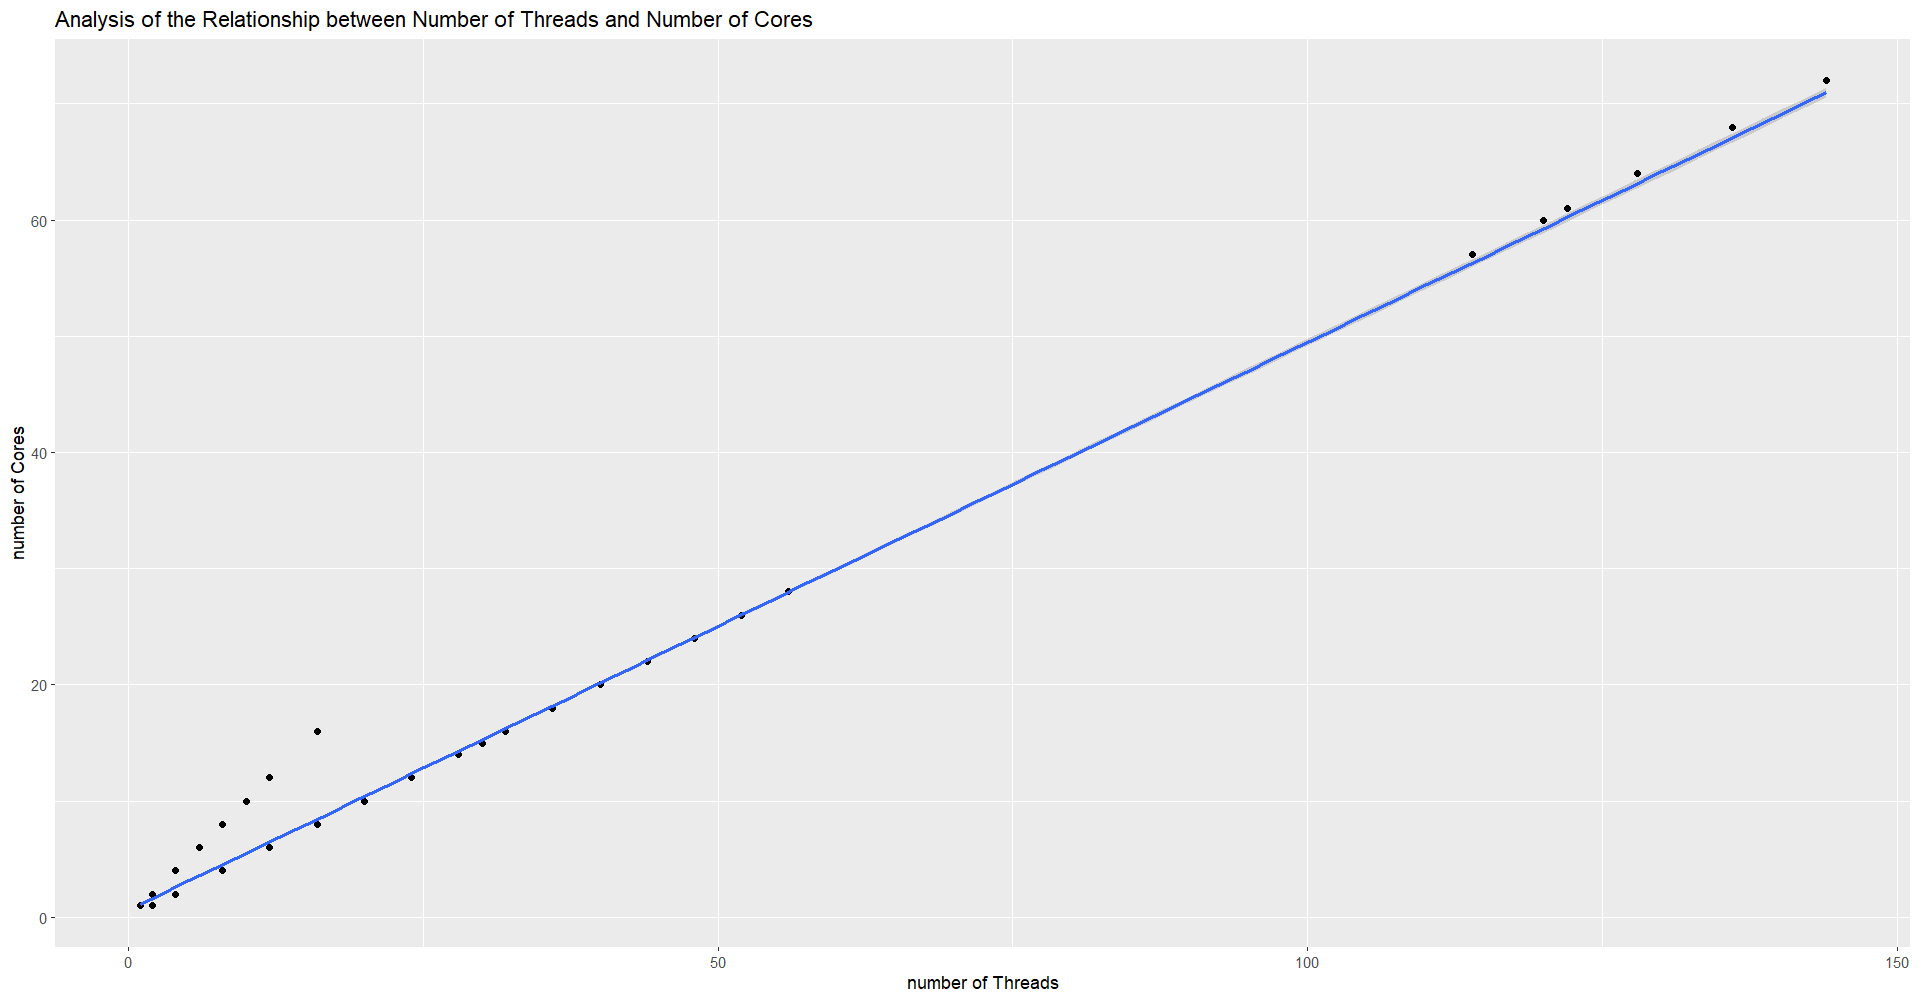
\includegraphics[width=1\linewidth]{img/CPU_ThreadCore.png}
  \vspace{1pt}
  \caption{Relation between Number of Threads and Number of Cores}
\end{figure}

\begin{figure}[ht]
  \centering
  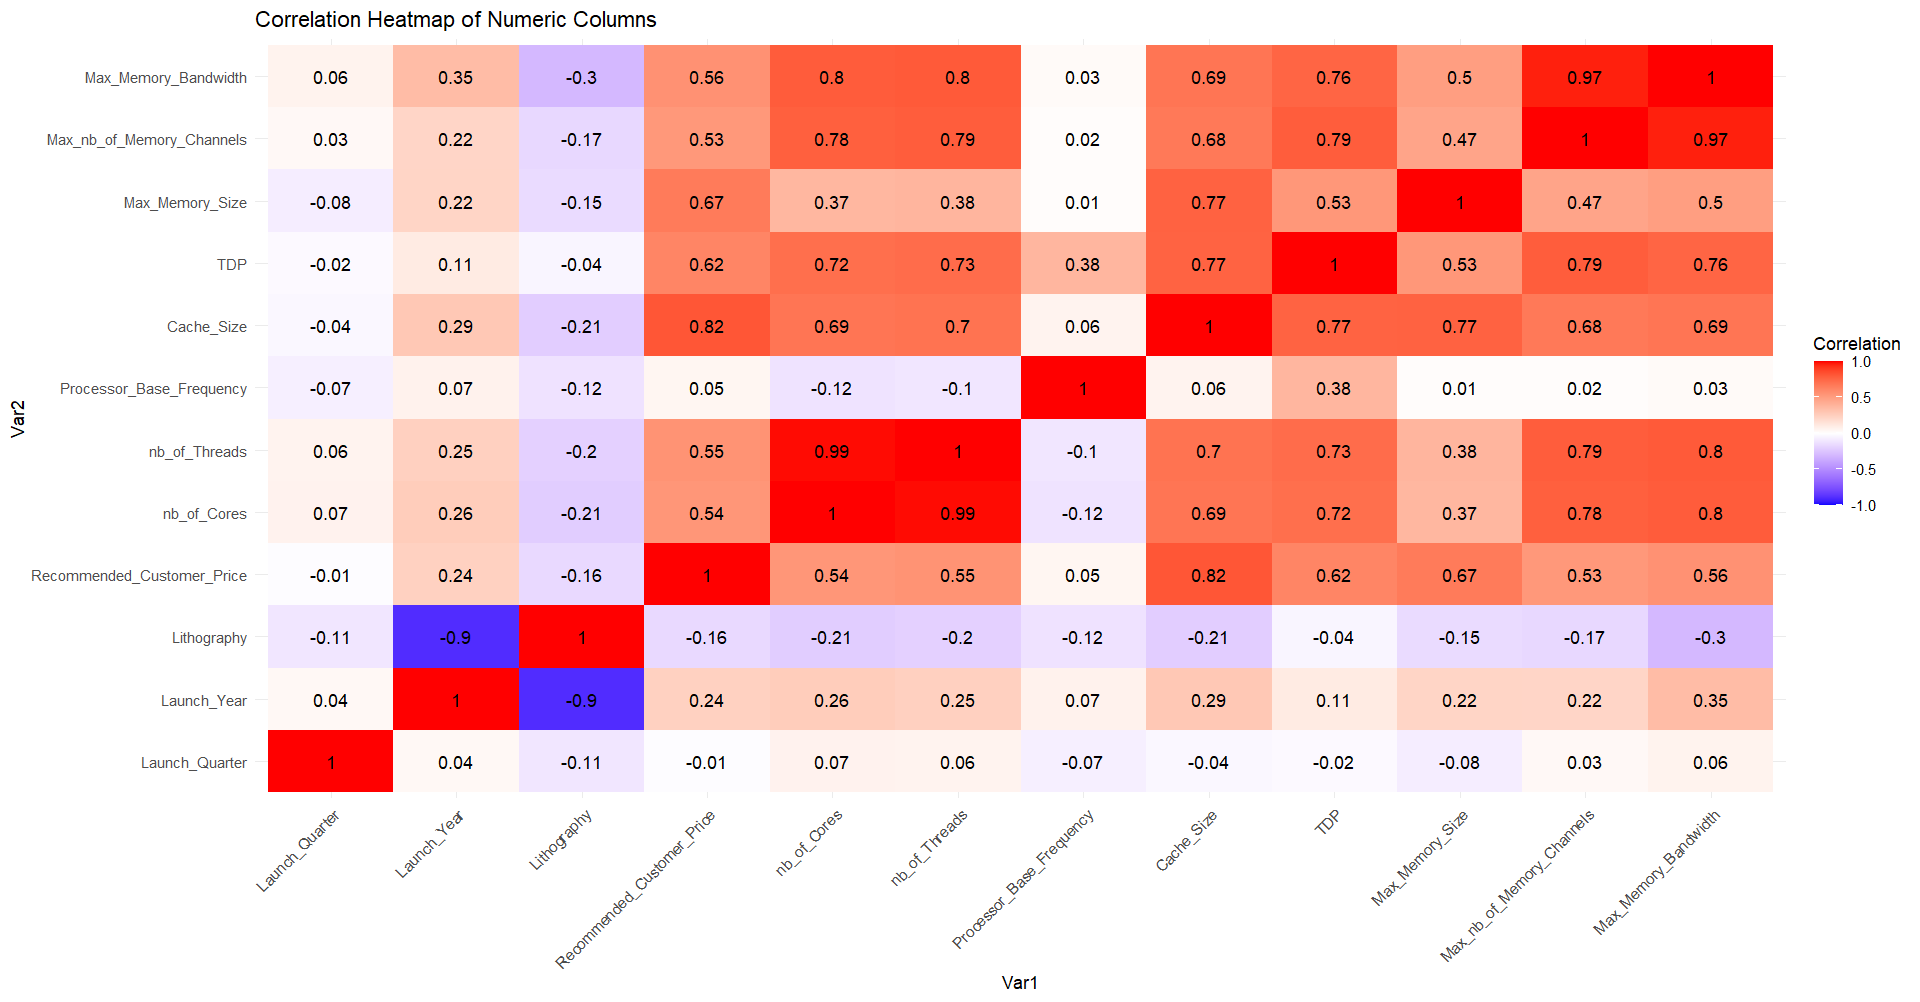
\includegraphics[width=1\linewidth]{img/CPU_cor.png}
  \vspace{1pt}
  \caption{Overall Correlation}
\end{figure}

\section{GPU Data}

\begin{lstlisting}[language=R]
freq <- table(GPUs_processed$Manufacturer, GPUs_processed$Release_Year)
total_count <- colSums(freq)
percentage <- prop.table(freq, margin = 2) * 100

barplot(freq,
        legend.text = TRUE,
        main = "Counts of Each Year",
        xlab = "Year",
        ylab = "Count",
        col = c("skyblue", "salmon", "lightgreen", "yellow"),
        border = "black")
\end{lstlisting}

\begin{figure}[ht]
  \centering
  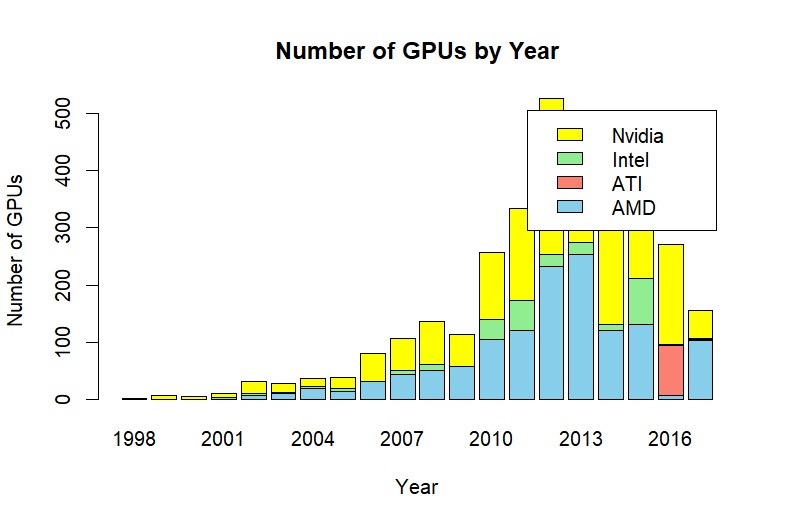
\includegraphics[width=1\linewidth]{img/Market_Year.png}
  \vspace{1pt}
  \caption{Sales of GPU manufacturer over years}
\end{figure}

\begin{lstlisting}[language=R]
barplot(percentage,
        legend.text = TRUE,
        main = "Market Share Percentage by Year",
        xlab = "Year",
        ylab = "Percentage",
        col = c("skyblue", "salmon", "lightgreen", "yellow"),
        border = "black")
\end{lstlisting}

\begin{figure}[ht]
  \centering
  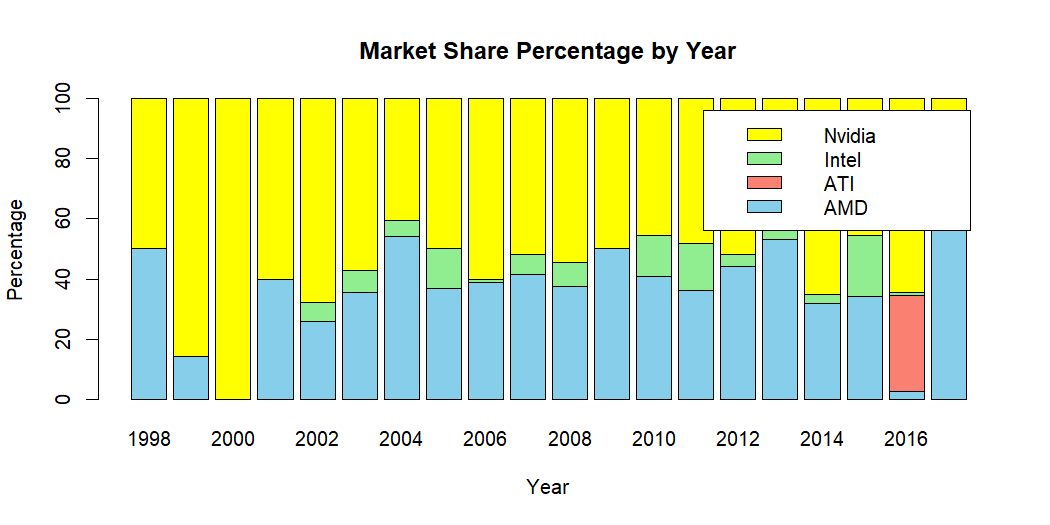
\includegraphics[width=1\linewidth]{img/Market_Percent_Year.png}
  \vspace{1pt}
  \caption{Market Share of GPU manufacturer over years}
\end{figure}

\begin{lstlisting}[language=R]
scatter_plot <- 
  ggplot(GPUs_processed, aes(x = Release_Year + Release_Month/12, y = Memory, color = Manufacturer)) +
  geom_point() +
  scale_color_manual(values = c("skyblue", "salmon", "lightgreen", "yellow")) +
  labs(x = "Year", y = "GPU Memory", title = "Scatter Plot of GPU Memory over Years") +
  theme_minimal()
print(scatter_plot)
\end{lstlisting}

\begin{figure}[ht]
  \centering
  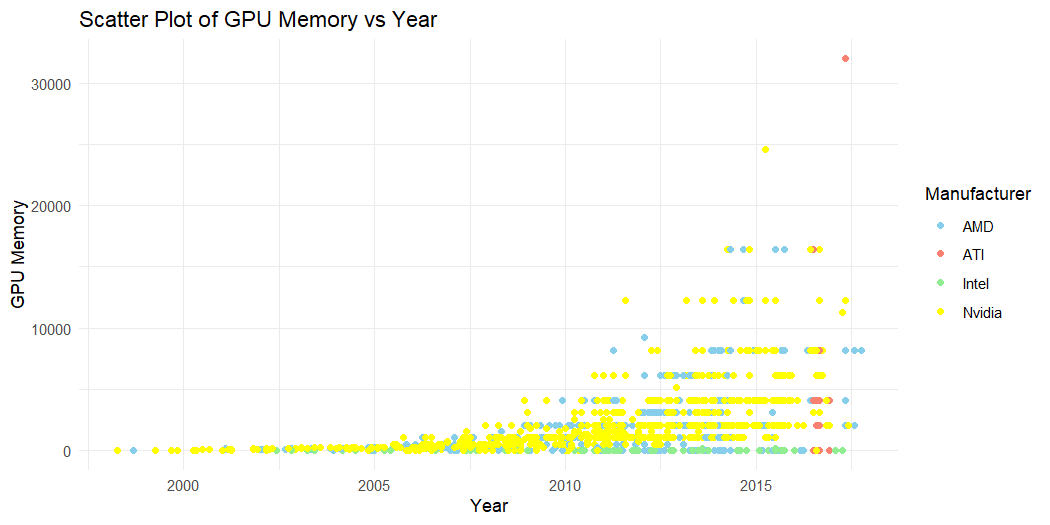
\includegraphics[width=1\linewidth]{img/GPU_Memo_Year.png}
  \vspace{1pt}
  \caption{GPU Memory over Years}
\end{figure}

\begin{lstlisting}[language=R]
memory_summary <- GPUs_processed %>%
  group_by(Release_Year) %>%
  summarise(mean_memory = mean(Memory),
            median_memory = median(Memory))

line_plot <- ggplot(memory_summary, aes(x = Release_Year)) +
  geom_line(aes(y = mean_memory, color = "Mean")) +
  geom_line(aes(y = median_memory, color = "Median")) +
  scale_color_manual(values = c("Mean" = "blue", "Median" = "red")) +
  labs(x = "Year", y = "Memory", title = "Mean and Median Memory by Year") +
  theme_minimal()
print(line_plot)
\end{lstlisting}

\begin{figure}[ht]
  \centering
  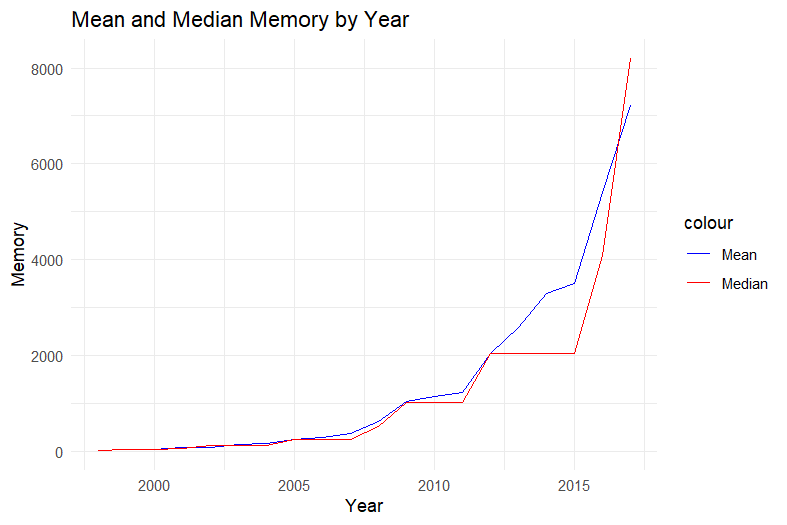
\includegraphics[width=1\linewidth]{img/MeaMedMem_Year.png}
  \vspace{1pt}
  \caption{Mean and median of memory over years}
\end{figure}

\begin{lstlisting}[language=R]
moore_law <- data.frame(
  Release_Year = seq(min(memory_summary$Release_Year), max(memory_summary$Release_Year), 1),
  Memory = 2^(0.5 * (seq(min(memory_summary$Release_Year), max(memory_summary$Release_Year), 1) - min(memory_summary$Release_Year - 8)))
)

memory_summary$log_mean_memory <- log(memory_summary$mean_memory)
memory_summary$log_median_memory <- log(memory_summary$median_memory)

line_plot <- ggplot(memory_summary, aes(x = Release_Year)) +
  geom_line(aes(y = log_mean_memory, color = "Logarithm of Mean"), size = 1) +
  geom_line(aes(y = log_median_memory, color = "Logarithm of Median"), size = 1) +
  geom_line(data = moore_law, aes(y = log(Memory), color = "Moore's Law"), size = 1, linetype = "dashed") +
  scale_color_manual(values = c("Logarithm of Mean" = "blue", "Logarithm of Median" = "red", "Moore's Law" = "green4")) +
  labs(x = "Year", y = "Logarithm of Memory", title = "Logarithm of Mean and Median Memory by Year") +
  theme_minimal()

print(line_plot)
\end{lstlisting}

\begin{figure}[ht]
  \centering
  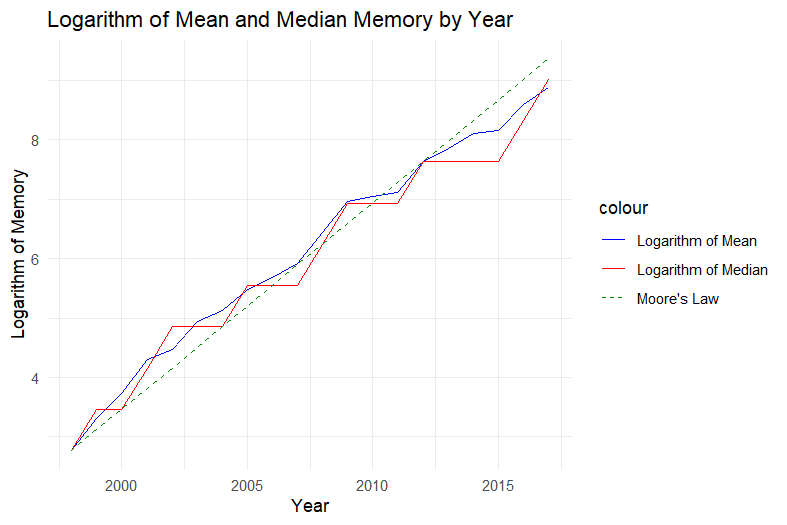
\includegraphics[width=1\linewidth]{img/LogMeaMedMem_Year.png}
  \vspace{1pt}
  \caption{Logarithm of Mean and Median Memory by Year}
\end{figure}


\begin{figure}[ht]
  \centering
  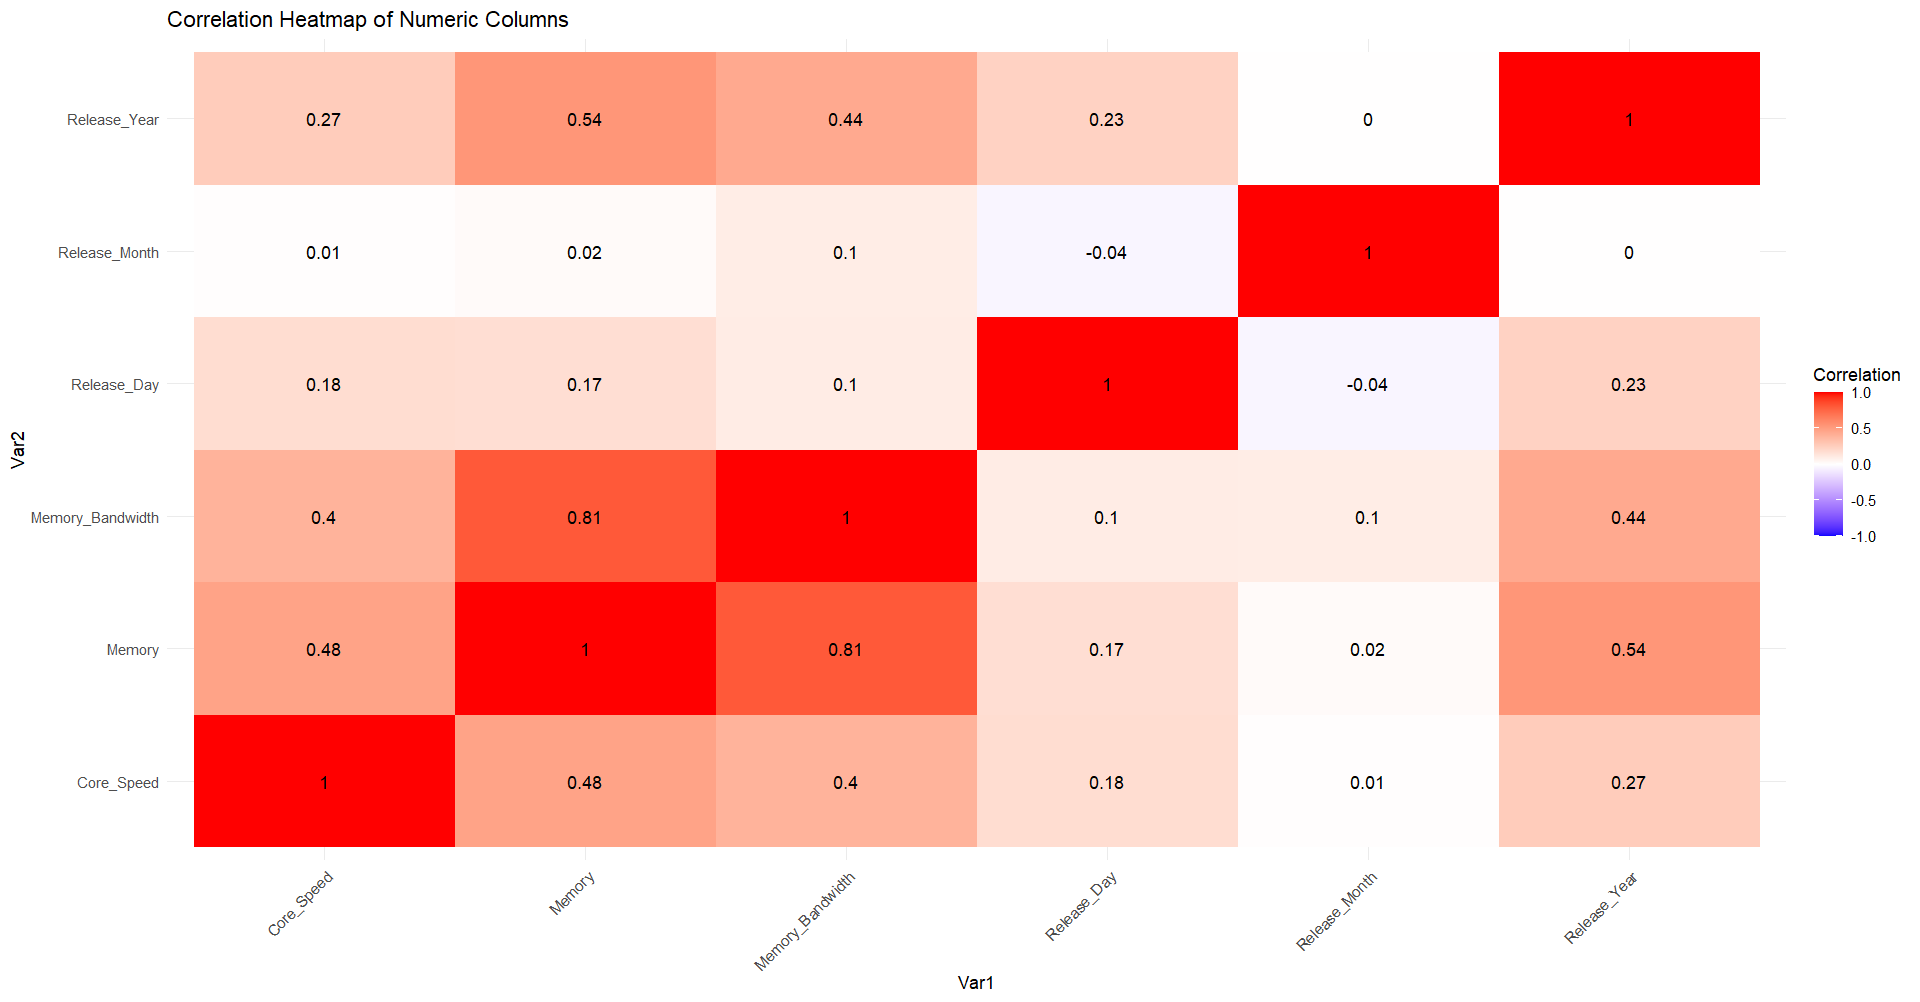
\includegraphics[width=1\linewidth]{img/GPU_cor.png}
  \vspace{1pt}
  \caption{Enter Caption}
\end{figure}
\chapter{Inferential Statistics}

\section{Two-way ANOVA}
\subsection{Problem Statement}

Many customers believe that the product lines in each applied segment will have different numbers of cores, so perform ANOVA testing to check if there is a relationship between \texttt{Product\_Collection} and \texttt{Vertical\_Segment} to \texttt{nb\_of\_Cores}.

\begin{figure}[ht]
  \centering
  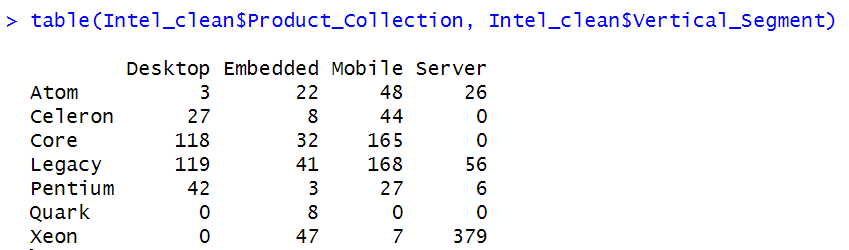
\includegraphics[width=14cm]{img/1.png}
  \caption{Data Partition based on \texttt{Product\_Collection} and \texttt{Vertical\_Segment}}
\end{figure}

\subsection{Hypotheses Testing}

\begin{lstlisting}[language=R]

  \end{lstlisting}

% Rút gọn tên biến, chuyển các yếu tố định tính về nhân tố thống kê (factor).
% \begin{figure}[h!]
%  \begin{left}
%   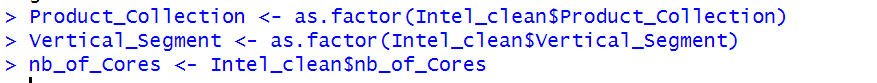
\includegraphics[width=12cm]{img/2.png}
%  \end{left}
% \end{figure}
% \\
% Kiểm tra dữ liệu nb\_of\_Cores có theo phân phối chuẩn hay không bằng Shapiro-Wilk test. \\
% Thư viện: \texttt{library(nortest)} \\
% Lệnh: \texttt{shapiro.test()} \\
% Giả thuyết:

% $H_0$: biến \texttt{nb\_of\_Cores} tuân theo phân phối chuẩn.

% $H_1$: biến \texttt{nb\_of\_Cores} không tuân theo phân phối chuẩn.
% \begin{figure}[h!]
%  \begin{left}
%   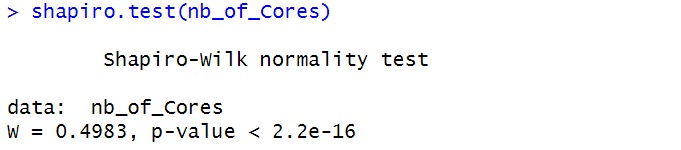
\includegraphics[width=12cm]{3.png}
%  \end{left}
% \end{figure} \\
% Nhận xét: p-value = $2.2 e-16 < 0.05$, ta bác bỏ giả thuyết $H_0$ hay nói cách khác biến \texttt{nb\_of\_Cores} không tuân theo phân phối chuẩn. \\
% Vẽ biểu đồ Q-Q Plot để có cái nhìn trực quan hơn về tính phân phối chuẩn của biến \texttt{nb\_of\_Cores}. \\
% Thư viện: \texttt{library(ggpubr)} \\
% Lệnh: \texttt{ggqqplot()}
% \begin{figure}[h!]
%  \begin{left}
%   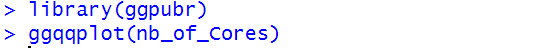
\includegraphics[width=12cm]{4.png}
%  \end{left}
% \end{figure} \\
% Kết quả:
% \begin{figure}[h!]
%  \begin{left}
%   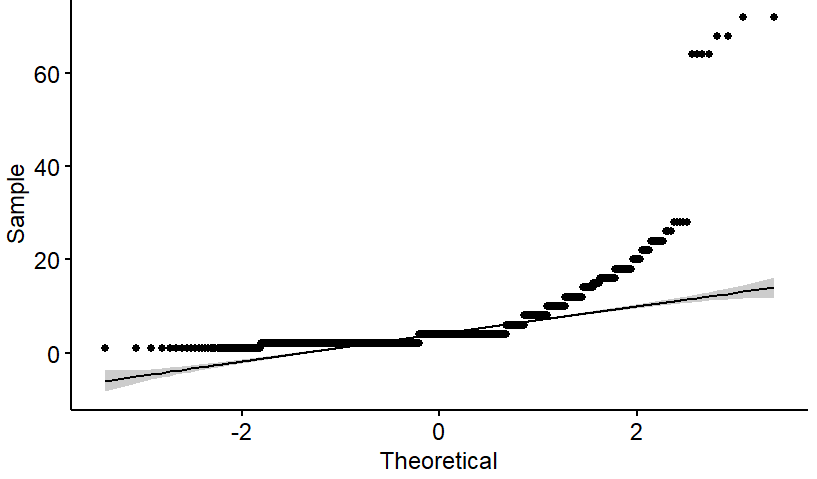
\includegraphics[width=15cm]{5.png}
%  \end{left}
% \end{figure} \\ \\ \\ \\ \\ \\
% Nhận xét: Biểu đồ QQ-plot cho ta thấy những giá trị quan sát đa phần không nằm trên đường thẳng kì vọng của phân phối chuẩn, do đó biến \texttt{nb\_of\_Cores} không tuân theo phân phối chuẩn. \\
% Kiểm định tính đồng nhất của phương sai dữ liệu bằng Levene's test.\\
% Thư viện: \texttt{library(car)}\\
% Lệnh: \texttt{leveneTest()}\\
% Giả thuyết:

% $H_0$: phương sai của các nhóm dữ liệu bằng nhau.

% $H_1$: tồn tại hai nhóm dữ liệu có phương sai khác nhau.
% \begin{figure}[h!]
%  \begin{left}
%   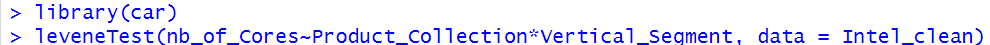
\includegraphics[width=15cm]{6.png}
%  \end{left}
% \end{figure} \\
% Kết quả:
% \begin{figure}[h!]
%  \begin{left}
%   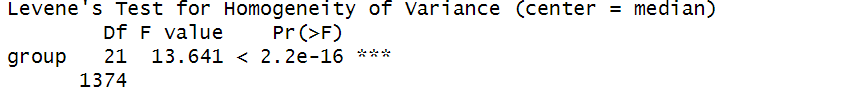
\includegraphics[width=12cm]{7.png}
%  \end{left}
% \end{figure}

% Nhận xét: $p\text{-value} < 2.2 e-16$ là rất nhỏ, nhỏ hơn 0.05, ta bác bỏ giả thuyết $H_0$ hay nói cách khác các nhóm dữ liệu có phương sai không đồng nhất.

% Kết luận: do dữ liệu \texttt{nb\_of\_Cores} không tuân theo phân phối chuẩn và các nhóm dữ liệu không có phương sai đồng nhất nên không thỏa mãn điều kiện bài toán Anova hai nhân tố. Nhưng do đây là một mẫu lớn nên ta có thể bỏ qua vi phạm này.

% Thực hiện phân tích Anova hai nhân tố:

% Mục đích: Kiểm tra sự ảnh hưởng của hai nhân tố \texttt{Product\_Collection} và \texttt{Vertical\_Segment} đối với \texttt{nb\_of\_Cores}.

% Do đây là một mẫu lớn nên dù mẫu đã vi phạm các giả định về phân phối chuẩn và phương sai đồng nhất thì phương pháp ANOVA hai nhân tố vẫn có thể áp dụng được. Tuy nhiên kết quả chỉ mang tính chất tham khảo, nếu muốn có kết quả chính xác hơn thì ta có thể sử dụng những phương pháp khác.

% Ta sẽ kiểm định các nhóm có số lượng mẫu lớn (>30).

% Chọn dữ liệu đầu vào:
% \begin{itemize}
%  \item \texttt{Product\_Collection}: Core, Legacy.
%  \item \texttt{Vertical\_Segment}: Desktop, Embedded, Mobile.
% \end{itemize}
% \newpage
% \begin{figure}[h!]
%  \begin{left}
%   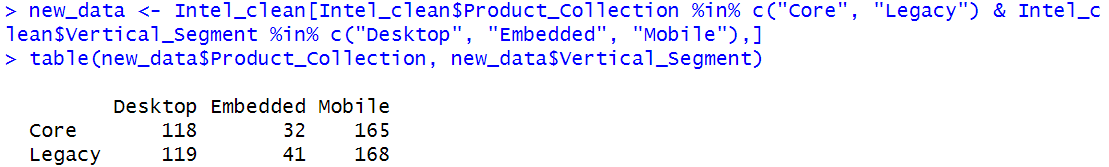
\includegraphics[width=15cm]{8.png}
%  \end{left}
% \end{figure} \\ \\ \\ \\ \\
% Rút gọn tên biến, chuyển các yếu tố định tính về nhân tố thống kê (factor).
% \begin{figure}[h!]
%  \begin{left}
%   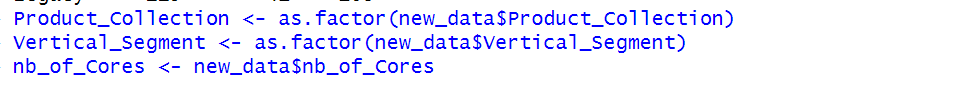
\includegraphics[width=15cm]{9.png}
%  \end{left}
% \end{figure} \\
% Dùng lệnh aov() để phân tích Anova rồi lưu kết quả vào av, để hiển thị kết quả ta dùng lệnh summary(av). \\
% Kết quả:
% \begin{figure}[h!]
%  \begin{left}
%   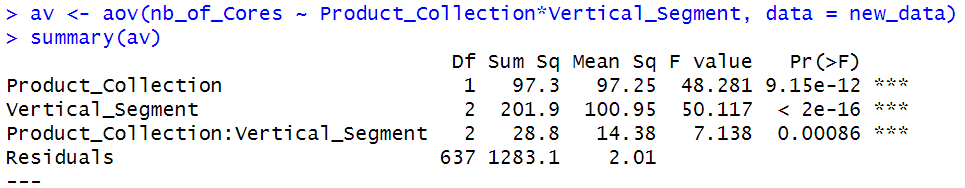
\includegraphics[width=12cm]{10.png}
%  \end{left}
% \end{figure} \\
% Trong kết quả trên, có các cột: Df (degrees of freedom) là bậc tự do; Sum Sq là tổng bình phương (sum of squares), Mean Sq là trung bình bình phương (mean square); F value là giá trị F; và Pr(>F) là trị số P liên quan đến kiểm định F. \\
% \textbf{Nhận xét:} Qua trung bình bình phương (Mean sq), chúng ta thấy ảnh hưởng của Product\_Collection và Vertical\_Segment có vẻ là như nhau, và cả hai ảnh hưởng đều có ý
% nghĩa thống kê, vì trị số p rất thấp cho hai yếu tố, cụ thể:\\
% \textbf{Đối với Product\_Collection:} \\
% Giả thuyết:

% $H_0$: số lõi CPU trung bình ở hai loại sản phẩm Core và Legacy là giống nhau.

% $H_1$: số lõi CPU trung bình ở hai loại sản phẩm Core và Legacy là khác nhau.
% \\
% Nhận xét: vì $p\text{-value} = 0.15 e-12 < 0.05$ nên ta bác bỏ giả thuyết $H_0$.\\
% \textbf{Đối với Vertical\_Segment:}\\
% Giả thuyết:

% $H_0$: số lõi CPU trung bình ở các phân khúc ứng dụng Desktop, Embedded, Mobile là giống nhau.

% $H_1$: có ít nhất hai phân khúc có số lõi CPU trung bình khác nhau.\\
% Nhận xét: vì $p\text{-value} < 2 e-16$ là rất nhỏ so với 0.05 nên ta bác bỏ giả thuyết $H_0$.\\
% \textbf{Kết luận:} số lõi CPU trung bình là khác nhau đối với các dòng sản phẩm (\texttt{Product\_Collection}) và phân khúc ứng dụng (\texttt{Vertical\_Segment}) khác nhau, nên số lõi CPU trung bình phụ thuộc vào dòng sản phẩm và phân khúc ứng dụng.

\chapter{Discussion}


\printindex
% \printbibliography
\end{document}